%% FEI-template.tex
%% Este trabalho utiliza uma adaptação da classe USPSC.cls que é mantida pela seguinte equipe:
%% 
%% Coordenação e Programação:
%%   - Marilza Aparecida Rodrigues Tognetti - marilza@sc.usp.br (PUSP-SC)
%%   - Ana Paula Aparecida Calabrez - aninha@sc.usp.br (PUSP-SC)
%% Normalização:
%%   - Brianda de Oliveira Ordonho Sigolo - brianda@usp.br (IAU)
%%   - Eduardo Graziosi Silva - edu.gs@sc.usp.br (EESC)
%%   - Eliana de Cássia Aquareli Cordeiro - eliana@iqsc.usp.br (IQSC)
%%   - Flávia Helena Cassin - cassinp@sc.usp.br (EESC)
%%   - Maria Cristina Cavarette Dziabas - mcdziaba@ifsc.usp.br (IFSC)
%%   - Regina Célia Vidal Medeiros - rcvmat@icmc.usp.br (ICMC)
%%



%----------------------------------------------------------------
%% Sobre a classe abntex2.cls:
%% abntex2.cls, v-1.9.5 laurocesar
%% Copyright 2012-2015 by abnTeX2 group at https://www.abntex.net.br/ 
%%
%----------------------------------------------------------------

\documentclass[
% -- opções da classe memoir --
12pt,		% tamanho da fonte
%openright,	% capítulos começam em pág ímpar (insere página vazia caso preciso)
oneside,  % para impressão em anverso (frente) e verso. Oposto a oneside - Nota: utilizar \imprimirfolhaderosto*
%oneside, % para impressão em páginas separadas (somente anverso) -  Nota: utilizar \imprimirfolhaderosto
% inclua uma % antes do comando twoside e exclua a % antes do oneside 
a4paper,			% tamanho do papel. 
% -- opções da classe abntex2 --
chapter=TITLE,		% títulos de capítulos convertidos em letras maiúsculas
% -- opções do pacote babel --
english,			% idioma adicional para hifenização
french,				% idioma adicional para hifenização
spanish,			% idioma adicional para hifenização
brazil				% o último idioma é o principal do documento
]{classe/USPSC}

% ---
% Pacotes básicos - Fundamentais 
% ---
\usepackage[T1]{fontenc}		% Seleção de códigos de fonte.
\usepackage[utf8]{inputenc}		% Codificação do documento (conversão automática dos acentos)
\usepackage{times}		    	% Usa a fonte Times New Roman							
\usepackage{lastpage}			% Usado pela Ficha catalográfica
\usepackage{indentfirst}		% Indenta o primeiro parágrafo de cada seção.
\usepackage{color}				% Controle das cores
\usepackage{graphicx}			% Inclusão de gráficos
\usepackage{float} 				% Fixa tabelas e figuras no local exato
\usepackage{chemfig}            % Para escrever reações químicas
\usepackage{chemmacros}         % Para escrever reações químicas
\usepackage{tikz}				% Para escrever reações químicas e outros
\usetikzlibrary{positioning}
\usepackage{microtype} 			% para melhorias de justificação
\usepackage{pdfpages}
\usepackage{makeidx}            % para gerar índice remissivo
\usepackage{hyphenat}          % Pacote para retirar a hifenizacao do texto
\usepackage[absolute]{textpos} % Pacote permite o posicionamento do texto
\usepackage{eso-pic}           % Pacote para incluir imagem de fundo
\usepackage{makebox}           % Pacote para criar caixa de texto
\usepackage{setspace}
\usepackage{caption}
\captionsetup[table]{justification=raggedright, singlelinecheck=false, width=\textwidth} % Alinha a legenda da tabela à esquerda
\captionsetup[quadro]{justification=raggedright, singlelinecheck=false, width=\textwidth} % Alinha a legenda da tabela à esquerda	
\captionsetup[figure]{justification=raggedright, singlelinecheck=false, width=\textwidth} % Alinha a legenda da tabela à esquerda	
% ---
% Pacotes de citações
% Citações padrão ABNT
% ---
% Sistemas de chamada: autor-data ou numérico.
% Sistema autor-data
\usepackage[alf, abnt-emphasize=bf, abnt-thesis-year=both, abnt-repeated-author-omit=no, abnt-last-names=abnt, abnt-etal-cite=3, abnt-etal-list=3, abnt-etal-text=it, abnt-and-type=e, abnt-doi=doi, abnt-url-package=none, abnt-verbatim-entry=no]{abntex2cite}
\bibliographystyle{classe/abntex2-alf-USPSC}


% Se o idioma for o inglês, inclua % no comando acima e exclua o % do comando abaixo
%\bibliographystyle{USPSC-classe/abntex2-alfeng-USPSC}


% Complementarmente, verifique as instruções abaixo sobre os Pacotes de Nota de rodapé
% ---
% Pacotes de Nota de rodapé
% Configurações de nota de rodapé


\renewcommand{\footnotesize}{\small} %Comando para diminuir a fonte das notas de rodapé
\renewcommand{\ABNTEXchapterfont}{\rmfamily}
\newcommand{\citefonte}[1]{\fontsize{10}{12}\selectfont\citeauthor{#1}, \citeyear{#1}} %Exibe como Autor,Ano em fonte 10 para Fontes de Tabelas, Quadros e Figuras


% ---
% Pacotes adicionais, usados apenas no âmbito do Modelo Canônico do abnteX2
% ---
\usepackage{lipsum}				% para geração de dummy text
% ---

% pacotes de tabelas
\usepackage{multicol}	% Suporte a mesclagens em colunas
\usepackage{multirow}	% Suporte a mesclagens em linhas
\usepackage{longtable}	% Tabelas com várias páginas
\usepackage{threeparttablex}    % notas no longtable
\usepackage{array}


% Pacotes para Overleaf
%\usepackage{showframe} % Para resolver "Underfull \hbox" e "Underfull \vbox"

% ----
% Compatibilização com a ABNT NBR 6023:2018 e 10520:2023
\usepackage{classe/ABNT6023-10520}
\usepackage[acronym]{glossaries}
\makeglossaries


% Os demais dados deverão ser fornecidos no arquivo FEI-pre-textual
% Configurações de aparência do PDF final
% alterando o aspecto da cor azul
\definecolor{blue}{RGB}{41,5,195}

% informações do PDF
\makeatletter
\hypersetup{
	pdftitle={xxxx}, 
	pdfauthor={lwila},
	pdfsubject={\imprimirpreambulo},
	pdfcreator={LaTeX with abnTeX2},
	colorlinks=true,       		% false: boxed links; true: colored links
	linkcolor=black,          	% color of internal links
	citecolor=black,        		% color of links to bibliography
	filecolor=black,      		% color of file links
	urlcolor=black,
	%Para habilitar as cores dos links, retire a % antes dos comandos abaixo e inclua a % antes das 4 linhas de comando acima 
	%linkcolor=blue,            	% color of internal links
	%citecolor=blue,        		% color of links to bibliography
	%filecolor=magenta,      		% color of file links
	%urlcolor=blue,
	bookmarksdepth=4	
}
\makeatother
% --- 

% O tamanho do parágrafo é dado por:
\setlength{\parindent}{1.3cm}

% ---
% compila o sumário e índice
\makeindex
% ---

% ----
% Início do documento
% ----
\begin{document}

% Seleciona o idioma do documento (conforme pacotes do babel)
\selectlanguage{brazil}
% Se o idioma do texto for inglês, inclua uma % antes do 
%      comando \selectlanguage{brazil} e 
%      retire a % antes do comando abaixo
%\selectlanguage{english}

% Retira espaço extra obsoleto entre as frases.
\frenchspacing 

% --- Formatação dos Títulos
\renewcommand{\ABNTEXchapterfontsize}{\fontsize{12}{12}\bfseries}
\renewcommand{\ABNTEXsectionfontsize}{\fontsize{12}{12}\normalfont}
\renewcommand{\ABNTEXsubsectionfontsize}{\fontsize{12}{12}\bfseries}
\renewcommand{\ABNTEXsubsubsectionfontsize}{\fontsize{12}{12}\bfseries\itshape}
\renewcommand{\ABNTEXsubsubsubsectionfontsize}{\fontsize{12}{12}\normalfont}

% ----------------------------------------------------------
% ELEMENTOS PRÉ-TEXTUAIS
% ----------------------------------------------------------
% ---
% Capa
% ---
\imprimircapa
% ---
% Folha de rosto
% (o * indica impressão em anverso (frente) e verso )
% ---
\imprimirfolhaderosto*
%\imprimirfolhaderosto
% ---
% ---
% Inserir a ficha catalográfica em pdf
% ---
% A biblioteca da sua Unidade lhe fornecerá um PDF com a ficha catalográfica definitiva. 
% Quando estiver com o documento, salve-o como PDF no diretório 
% do seu projeto como fichacatalografica.pdf e inclua o arquivo 
% utilizando o comando abaixo:
 
%\includepdf{PreTextual/fichacatalografica.pdf}

% Se você optar por elaborar a ficha catalográfica, deverá 
%  retirar o % do comando abaixo
%% USPSC-fichacatalografica.tex
% ---
% Inserir a ficha bibliografica
% ---

\begin{center}
\large{A ficha catalográfica deve ser gerada automaticamente neste link: 
\url{https://ficha.fei.edu.br/ficha/?_gl=1*1wyaveq*_gcl_au*MTY2MDUzNTY0OC4xNzMwMjI1MzEw*_ga*MTc3NDA5MjgwOC4xNzIyNDQ3NzE5*_ga_9CWNLCJN1W*MTczMjg5ODUxNC40NjcuMS4xNzMyODk4NTE2LjU4LjAuMA}}
\end{center}

% As informações que compõem a ficha catalográfica estão 

% ---
% Inserir folha de aprovação
% ---

% A Folha de aprovação é um elemento obrigatório da NBR 4724/2011 (seção 4.2.1.3). 
% Após a defesa/aprovação do trabalho, gere o arquivo folhadeaprovacao.pdf da página assinada pela banca pelo Ábaris
% e iclua o arquivo utilizando o comando abaixo:
%\includepdf{PreTextual/folhadeaprovacao.pdf}

% Alternativa para a Folha de Aprovação:
% Se for a sua opção elaborar uma folha de aprovação, insira uma % antes do comando acima que inclui o arquivo folhadeaprovacao.pdf,
% tire o % do comando abaixo e altere o arquivo folhadeaprovacao.tex conforme suas necessidades
%% USPSC-folhadeaprovacao.tex
% Alternativa para a Folha de Aprovação 
% Se esta for a sua opção, exclua inclusão feita acima do arquivo folhadeaprovacao.pdf
%
\begin{folhadeaprovacao}
  \begin{center}
       {\ABNTEXchapterfont\normalfont\imprimirautor}\\
\textbf{PARA PÓS-GRADUAÇÃO, SUBSTITUIR ESSA  FOLHA DE APROVAÇÃO  PELA FOLHA ATA}
	 \vspace*{2cm}
   
    \begin{center}
      \ABNTEXchapterfont\bfseries\MakeUppercase\imprimirtitulo

    \end{center}
		\vspace*{3cm}
		\hspace{.45\textwidth}
    \begin{minipage}{.5\textwidth}
        \imprimirpreambulo
    \end{minipage}
		\vspace*{2cm}
    %\vspace*{\fill}
	\end{center}

  \begin{center}
		
	  {\ABNTEXchapterfont\normalfont\ {Comiss\~ao Julgadora:} \\}
		%Trabalho aprovado. \imprimirlocal, 2 de outubro de 2015:
		
		%\assinatura{\textbf{\imprimirorientador} \\ Orientador} 
		%\assinatura{\textbf{\imprimirorientador} \\}
    % Se for ORIENTADOR, inclua % no início do comando abaixo e tire a % do próximo comando 
		%\renewcommand{\orientadorname}{Orientadora}
		%\renewcommand{\orientadorname}{Orientador}

		\assinatura{Nome Orientador}
		
		\assinatura{Professor 1}
		
		\assinatura{Professor 2}
		%\assinatura{\textbf{Professor} \\ Convidado3}
		%\assinatura{\textbf{Professor} \\ Convidado4}
		%\begin{center}
		\vspace*{4cm}
   	{\ABNTEXchapterfont\normalfont\imprimirlocal}
    \par
%Adicionar data de aprovação da Banca
  {\ABNTEXchapterfont\normalfont\ {02 de outubro de XXXX} \\}
\end{center}
\end{folhadeaprovacao}
% ---

% ---
% Dedicatória
% ---
%% USPSC-Dedicatoria.tex
\begin{dedicatoria}
 \vspace*{20cm}
\noindent\hspace{8cm} % Recuo de 8 cm à esquerda
\begin{minipage}{8cm} % Define a largura do texto
    {\setlength{\baselineskip}{1.5\baselineskip} % Espaçamento de 1,5 entre linhas
    \noindent % Garantir alinhamento inicial
    {Espaço reservado para a dedicatória,justificado com 8cm de recuo à esquerda, com espaçamento entre linhas 1,5.}}
\end{minipage}

\end{dedicatoria}
% ---
% ---

% ---
% Agradecimentos
% ---
%% USPSC-Agradecimentos.tex

\begin{agradecimentos}
\vspace{-\baselineskip} %Manter para garantir o espaçamento da biblioteca.
Espaço reservado para os agradecimentos. Iniciado com parágrafo de 1,25. Espaçamento entre linhas 1,5.
\end{agradecimentos}
% ---
% ---

% ---
% Epígrafe
% ---
%% USPSC-Epigrafe.tex
\begin{epigrafe}
 \vspace*{20cm}
\noindent\hspace{8cm} % Recuo de 8 cm à esquerda
\begin{minipage}{8cm} % Define a largura do texto
    {\setlength{\baselineskip}{1.5\baselineskip} % Espaçamento de 1,5 entre linhas
    \noindent % Garantir alinhamento inicial
    {Espaço reservado para a epígrafe (apresentar entre aspas, digitada em espaço 1, 5 entre linhas, 8 cm de recuo à esquerda e justificada.  Acrescentar na lista de referências).}}
\end{minipage}
\end{epigrafe}
% ---
% ---

% A T E N Ç Ã O
% Se o idioma do texto for em inglês, o abstract deve preceder o resumo
% resumo em português
%
% Resumo
% ---
%% USPSC-Resumo.tex

\begin{resumo}
\setlength{\baselineskip}{1.5\baselineskip} % Espaçamento de 1,5 entre linhas

Elaborado pelo próprio autor, apresentação concisa dos pontos relevantes de um documento. Deve ressaltar o objetivo, o método, os resultados e as conclusões do documento. O resumo deve ser composto de uma sequência de frases concisas, afirmativas e não de enumeração de tópicos, deve ter alinhamento justificado em um único parágrafo (1,25 cm), espaçamento 1,5 entre linhas e deve-se usar o verbo na voz ativa e na terceira pessoa do singular. De acordo com a NBR 6028: 2003 –Informação e documentação – Resumo – Apresentação quanto a sua extensão os resumos devem ter: de 150 a 500 palavras para os trabalhos acadêmicos (teses, dissertações e outros) e relatórios técnico-científicos. 

   \vspace{\onelineskip}
\noindent
Palavras-chave: primeira; segunda; terceira. 

\end{resumo}
% ---

% Abstract
% ---
%% USPSC-Abstract.tex
%\autor{Silva, M. J.}
\begin{resumo}[Abstract]

\setlength{\baselineskip}{1.5\baselineskip} % Espaçamento de 1,5 entre linhas

The increasing availability of medical imaging exams, such as magnetic resonance imaging, generates a large volume of data, making its analysis complex and challenging. In this scenario, advanced computational approaches can optimize the interpretation of these images and assist in the early diagnosis of cardiovascular diseases. This work aims to unify contemporary approaches in the evaluation of cardiomyopathy. With the support of radiomic analysis, which extracts information from the statistical and texture characteristics of a medical image, and features derived from a classical neural network for computer vision, such as ResNet50, promising results can be obtained. The results confirm that the combination of information from various domains regarding a given patient, when integrated, can lead to more interesting outcomes compared to analyzing data in isolation. This study aims to apply the aforementioned approaches, based on previous literature, in an innovative application for cardiomyopathy testing, adapting and proposing a more robust architecture to achieve better results.

\vspace{\onelineskip}
\noindent 
Keywords: Radiomics; Attention Mechanism; Transformers; Cardiomyopathy.

\end{resumo}

% ---

% ---
% inserir lista de figurass
% ---

%Inserir Lista de Figuras --- COMENTAR TRECHO ABAIXO  EM CASO DE MENOS DE 5 FIGURAS
\pdfbookmark[0]{\listfigurename}{lof}
\listoffigures*
\cleardoublepage


% ---
% inserir lista de tabelas ----- COMENTAR TRECHO ABAIXO  EM CASO DE MENOS DE 5 TABELAS
% ---
\pdfbookmark[0]{\listtablename}{lot}
\listoftables*
\cleardoublepage
% ---

% ---
% inserir lista de quadros ---- COMENTAR TRECHO ABAIXO  EM CASO DE MENOS DE 5 QUADROS
% ---
\pdfbookmark[0]{\listofquadroname}{loq}
\listofquadro*
\cleardoublepage
% ---

% ---
% inserir lista de abreviaturas e siglas ----COMENTAR TRECHO ABAIXO  EM CASO DE MENOS DE 5 ABREVIATURAS
% USPSC-AbreviaturasSiglas.tex
\begin{siglas}
    \item[ABNT] Associação Brasileira de Normas Técnicas
    \item[abnTeX] ABsurdas Normas para TeX
	\item[IBGE] Instituto Brasileiro de Geografia e Estatística
	\item[LaTeX] Lamport TeX
	\item[USP] Universidade de São Paulo
	\item[USPSC] Campus USP de São Carlos
\end{siglas}

% ---

% ---
% inserir lista de símbolos -----COMENTAR TRECHO ABAIXO  EM CASO DE MENOS DE 5 SIMBOLOS
% USPSC-Simbolos.tex
\begin{simbolos}
  \item[$ \Gamma $] Letra grega Gama
  \item[$ \Lambda $] Lambda
  \item[$ \zeta $] Letra grega minúscula zeta
  \item[$ \in $] Pertence
\end{simbolos}
% ---
% ---
% inserir o sumario
% ---

\pdfbookmark[0]{\contentsname}{toc}
\tableofcontents*
\cleardoublepage
% ---
% ----------------------------------------------------------
% ELEMENTOS TEXTUAIS
% ----------------------------------------------------------
\textual
% Os capítulos são inseridos como arquivos externos 

% Capítulo 1 - Introdução
% ---
%% USPSC-Introducao.tex

% ----------------------------------------------------------
% Introdução (exemplo de capítulo sem numeração, mas presente no Sumário)
% ----------------------------------------------------------
\chapter[Introdução]{Introdução}
\label{chap:introducao}
\vspace{-\baselineskip} %Manter para garantir o espaçamento da biblioteca.

A tecnologia está cada vez mais presente nas diversas áreas do conhecimento, trazendo uma infinidade de benefícios e facilitando o cotidiano contemporâneo. Entre os diversos campos impactados, a área médica destaca-se como uma das que mais se beneficiaram da inovação tecnológica. Desde meados dos anos 2000, a quantidade de dados gerados na medicina tem crescido exponencialmente, atingindo projeções de milhares de \textit{exabytes} a partir de 2020 \cite{gantzDIGITALUNIVERSE2020}. Esse cenário evidencia a importância de ferramentas que possam processar e analisar eficientemente grandes volumes de informações.

Exames de imagem, como a \gls{tc} e a \gls{rmc}, tornaram-se essenciais na medicina moderna. Esses exames não apenas oferecem uma representação tridimensional detalhada de estruturas do corpo humano, mas também produzem dados que podem ser analisados de forma quantitativa. Em paralelo, a \gls{ia} trouxe avanços significativos à análise de imagens diagnósticas, proporcionando maior eficiência e precisão nos diagnósticos médicos \cite{argentieroApplicationsArtificialIntelligence2022}.

Nesse sentido, as redes neurais profundas, um dos principais pilares da \gls{ia}, têm demonstrado alto desempenho em tarefas de visão computacional, como classificação de imagens, detecção de objetos e segmentação. Essas redes conseguem aprender características discriminantes uma vez otimizadas a cerca do conjunto de dados em que foi treinada. Além disso, arquiteturas como o \textit{transformers} ficaram populares por serem comumente usadas em redes generativas auto-regressivas para geração sintética de texto, também conhecidas como \gls{llm}, tendo como como seu exemplo mais conhecido o \textit{ChatGPT}. Os \textit{transformers} são arquiteturas que destacam-se pela capacidade de paralelismo e pelo uso de mecanismos de autoatenção, que permitem ao modelo focar nas partes mais relevantes dos dados de entrada \cite{russell2020artificial}.

Adicionalmente, técnicas de processamento de imagem como a análise de textura já vem sendo utilizada por várias décadas em diversos domínios da medicina. A análise radiômica emergiu como uma ferramenta poderosa na extração de informações quantitativas de imagens médicas, capturando padrões que muitas vezes passam despercebidos ao olho humano. Essa abordagem tem mostrado potencial em diversas áreas, como oncologia e cardiologia \cite{schofieldTextureAnalysisCardiovascular2019a}.

No domínio da análise de imagens cardíacas, a análise de textura aplicada à \gls{rmc} tem avaliado o risco de arritmia pós-infarto do miocárdio. O uso de análise de textura para \gls{rmc} em imagens sem contraste e com realce tardio de gadolínio em pacientes com cardiomiopatia para prever o resultado do exame é uma área particular de interesse \cite{schofieldTextureAnalysisCardiovascular2019a}.

A \gls{cmh} é uma das cardiomiopatias mais comuns, frequentemente diagnosticada em jovens e indivíduos de meia-idade. Embora em muitos casos seja assintomática, a doença pode levar a condições graves, como insuficiência cardíaca e acidente vascular cerebral. Isso torna o diagnóstico precoce essencial para prevenir desfechos adversos \cite{kwonComparisonMortalityCause2022}. Neste sentido a análise radiômica que consiste em extrair dados qualitativos de imagens médicas, incluindo, em muitos casos, a análise da textura dessas imagens \cite{lambinRadiomicsExtractingMore2012}. A análise radiômica pode auxiliar com o diagnóstico prévio afim de compreender e atuar nos casos de cardiomiopatia que demonstrem risco ao paciente.

Neste cenário, combinar técnicas de \gls{ia} e análise radiômica representa uma estratégia promissora para a detecção de cardiomiopatias entre outras condições cardíacas. Estudos recentes, como o de \citeonline{aiSelfAttentionBasedFusion2023}, demonstraram que a integração de características profundas e radiômicas podem melhorar significativamente o desempenho preditivo de modelos diagnósticos de câncer de pulmão via imagens de \gls{tc}. Esses modelos baseiam-se em mecanismos de autoatenção para identificar padrões relevantes em dados concatenados, alcançando acurácia de até $82,35\%$ e \gls{auc} de $0,74$.

Assim, o presente trabalho propõe a implementação e validação de uma estratégia de fusão que combine características radiômicas e profundas, com o uso de mecanismos de autoatenção, para melhorar a classificação de cardiomiopatias. Além de avançar o estado da arte em diagnósticos médicos, esta pesquisa busca contribuir para a adoção de soluções mais eficazes e acessíveis no apoio à decisão clínica.

%---------------------------------------------------------
\section{OBJETIVOS}
\label{sec:cap1_objetivo}

Os objetivos deste trabalho consistem em propor e validar uma abordagem inovadora para a classificação de cardiomiopatias utilizando técnicas de inteligência artificial e análise radiômica. Estes objetivos foram definidos para responder às necessidades clínicas e avançar o estado da arte na área de diagnóstico médico. Com isso, o objetivo geral do presente projeto é desenvolver, implementar e validar um modelo de classificação de cardiomiopatias, utilizando a integração de características radiômicas e profundas mediadas por mecanismos de autoatenção. Os objetivos específicos, por sua vez, são elencados conforme os itens abaixo:


\begin{enumerate}
\item Identificar e extrair características radiômicas de imagens de \gls{rmc}, capturando padrões texturais e estatísticos relevantes para a classificação das cardiomiopatias.

\item Projetar um pipeline de análise que combine eficientemente características radiômicas e profundas, garantindo a fusão informativa para modelos de aprendizado profundo.

\item Implementar um modelo baseado em redes neurais profundas que utilize mecanismos de atenção para priorizar regiões relevantes nas imagens, melhorando a acurácia e a interpretabilidade do modelo.

\item Validar a eficácia do modelo proposto utilizando métricas padrão, como acurácia, precisão, revocação, F1-score e \gls{auc}, em um conjunto de dados públicos e diversificado.

\item Comparar o desempenho do modelo proposto com técnicas existentes na literatura, identificando avanços e limitações em relação às abordagens tradicionais.
\end{enumerate}


%---------------------------------------------------------
\section{ESTRUTURA DO TRABALHO}
\label{sec:cap1_estrutura_trabalho}

Este trabalho está organizado em sete capítulos, cada um projetado para abordar diferentes aspectos da pesquisa e sua implementação. A seguir, apresenta-se a estrutura detalhada desta pesquisa:

O \textbf{Capítulo \ref{chap:introducao}} apresenta o contexto geral do trabalho, destacando a relevância do uso de inteligência artificial e análise radiômica no diagnóstico de cardiomiopatias. São expostos os objetivos gerais e específicos da pesquisa, bem como a motivação para o desenvolvimento deste estudo. O \textbf{Capítulo \ref{chap:fundamentacao_teorica}} discute os conceitos teóricos que embasam o trabalho, incluindo princípios de redes neurais profundas, análise radiômica, mecanismos de autoatenção e sua aplicação em imagens médicas. Este capítulo também revisa estudos relacionados que contribuíram para o estado da arte na área. No \textbf{Capítulo \ref{chap:trab_relacionados}} é estudado  os trabalhos recentes, não superior a cinco anos passados, de outros autores que estão de alguma forma relacionados com tema, sendo estes trabalhos relacionados oriundos de uma minuciosa revisão sistemática da literatura. O \textbf{Capítulo \ref{chap:metodologia}} detalha o método proposto para a classificação de cardiomiopatias, incluindo a descrição do conjunto de dados utilizado, o processo de extração de características radiômicas, o desenvolvimento do modelo baseado em redes neurais profundas e as etapas de validação e experimentação. O \textbf{Capítulo \ref{chap:proposta_experimental}} faz a proposição experimental que contempla os dados utilizados, informações do seu pré-processamento, hiperparâmetros planejados e demais informações a cerca do experimentos realizados. Neste capítulo também é apresentado os resultados obtidos com a implementação do modelo proposto, acompanhados de análises quantitativas e qualitativas. Discute-se o desempenho do modelo em comparação com outras abordagens e suas implicações técnicas. Finalmente, o \textbf{Capítulo \ref{chap:cap7_conclusao}} sintetiza os principais achados da pesquisa, destacando as contribuições do trabalho para o estado da arte e suas potenciais aplicações. Além disso, são sugeridas direções para estudos futuros que possam expandir e aprimorar as técnicas apresentadas.

% ---

% ---
% Capítulo 2
% ---
%% USPSC-Cap2-Desenvolvimento.tex 

% ---
% Este capítulo, utilizado por diferentes exemplos do abnTeX2, ilustra o uso de
% comandos do abnTeX2 e de LaTeX.
% ---

\chapter{Fundamentação Teórica}
\label{chap:fundamentacao_teorica}
\vspace{-\baselineskip} %Manter para garantir o espaçamento da biblioteca.

A proposta deste trabalho visa unificar informações das características radiômicas e características profundas oriundas de uma rede neural convolucional e, por conseguinte, propor uma arquitetura de autoatenção para identificar características discriminantes a fim de obter resultados relevantes na classificação de cardiomiopatias.

%--------------------------------------------------------
\section{RESSONÂNCIA MAGNÉTICA EM CARDIOMIOPATIA}
\label{sec:rmc}

A \gls{rmc} se tornou um dos principais métodos em imagem médica para avaliar a fisiologia e a função na doença cardíaca congênita. A \gls{rmc} possui funções que normalmente são obtidas por ecocardiografia, tendo como exemplo a velocidade média em um vaso, mas também apresenta características muito especiais como calcular a velocidade em um voxel de um milímetro em qualquer lugar no espaço tridimensional do vaso.
Usando a tecnologia atual de \gls{rmc}, os investigadores podem obter percepções únicas sobre a função ventricular, por exemplo, deformação ventricular regional \textit{in vivo}, movimento da parede e mecânica dos fluidos, por exemplo, visualização \textit{in vivo} de perfis de velocidade além de aumentar a precisão de medidas padrão aceitas pela fisiologia ou função ventricular, por exemplo, débito cardíaco, volumes ventriculares e massa. Devido ao rápido avanço da tecnologia, muitas técnicas de \gls{rmc} são experimentais ou ainda estão em fase de desenvolvimento clínico; no entanto, há muitas técnicas que são clinicamente úteis, por exemplo, medição do volume ventricular em pacientes com tamanho ventricular esquerdo limítrofe. Como muitas das técnicas experimentais atuais serão, sem dúvida, empregadas na prática clínica no futuro, os médicos devem estar cientes de todo o espectro de capacidades da \gls{rmc} \cite{fogelAssessmentCardiacFunction2000}.

Em muitos cenários clínicos, as limitações técnicas da ecocardiografia e a expressão fenotípica heterogênea tornaram tal avaliação difícil e a \gls{rmc} emergiu como uma modalidade de imagem complementar útil para incorporar a ecocardiografia transtorácica de rotina. A \gls{rmc} cardíaca é única em sua alta resolução espacial e temporal com excelente contraste entre o \textit{pool} sanguíneo e o miocárdio, sem limitação de janela de imagem ou plano de imagem.
A heterogeneidade fenotípica da miocardiopatia hipertrófica é bem reconhecida pela dificuldade em sua identificação. Isto se complica ainda mais pois nem todos os pacientes com hipertrofia ventricular esquerda têm \gls{cmh}, enquanto uma fisiopatologia semelhante à \gls{cmh} com obstrução dinâmica do trato de saída do ventrículo esquerdo pode ser observada sem hipertrofia do ventrículo esquerdo, em um subgrupo de pacientes com anormalidades na válvula mitral e/ou no músculo papilar \cite{pontoneClinicalApplicationsCardiac2022}.

A \gls{cmh} é uma doença heterogênea com expressão morfológica complexa que requer uma caracterização precisa da doença para um planejamento terapêutico ótimo e estratificação de risco. A \gls{rmc} cardíaca emergiu como um complemento útil para esses propósitos. Com a incorporação crescente de imagem multimodal na avaliação clínica da \gls{cmh}, o entendimento sobre a importância de diferenças morfológicas sutis continuará a crescer, e pesquisas adicionais definirão novos marcadores prognósticos e melhorarão as estratégias de tratamentos atuais \cite{toCardiacMagneticResonance2011c}.

%--------------------------------------------------------
\section{ANÁLISE RADIÔMICA}
\label{sec:analise_radiomica}

A análise radiômica é um campo de pesquisa em rápida evolução, preocupada com a extração de informações quantitativas, incluindo padrões complexos que são difíceis de reconhecer ou quantificar pelo olho humano a cerca de imagens médicas, características estas chamadas de características radiômicas. As características radiômicas podem capturar características de tecidos e lesões, como forma e heterogeneidade, e podem, sozinhas ou em combinação com dados demográficos, histológicos, genômicos ou proteômicos, ser usadas para a resolução de problemas clínicos.

Mesmo que características radiômicas individuais podem se correlacionar com dados genômicos ou dados clínicos, o impacto da análise radiômica se torna mais relevante a medida que mais informações são por ela extraídas. Tipicamente centenas de características, uma fração do total que é extraído, contribuem para identificação de uma doença específica e é processada usando técnicas de aprendizado de máquina. As características radiômicas podem ser subdivididas em estatísticas, incluindo as baseadas em histograma e textura; modelo; transformação; e forma. A extração pode ser dada em regiões de interesse de 2-dimensões (2D) e 3-dimensões (3D)  \cite{mayerhoeferIntroductionRadiomics2020}.


%--------------------------------------------------------
\subsection{Características por Histograma}

Os descritores estatísticos mais simples são baseados no histograma global de níveis de cinza e incluem média de nível de cinza, máximo, mínimo, variância e percentis. Como essas características são baseadas em análises de \textit{pixel} único ou \textit{voxel} único (3D), elas são chamadas de características de primeira ordem. Algumas características mais sofisticadas incluem assimetria e curtose que descrevem a forma da distribuição da intensidade dos dados: a assimetria reflete a assimetria da curva da distribuição de dados para a esquerda (assimetria negativa, abaixo da média) ou direita (assimetria positiva, acima da média), enquanto a curtose reflete a caudalidade de uma distribuição de dados em relação a uma distribuição gaussiana devido a \textit{outliers}. Outras características incluem histograma entrópico e uniformidade, e também é comumente chamado de energia.

%--------------------------------------------------------
\subsection{Características de Textura}

Uma abordagem simples para a descrição de textura radiômica é a análise do gradiente absoluto, que reflete o grau ou a abruptidade das flutuações de intensidade de nível de cinza em uma imagem. Para dois \textit{pixels} ou \textit{voxels} adjacentes, o gradiente é o máximo possível quando um for preto e o outro branco, enquanto se ambos os \textit{pixels} forem pretos (ou ambos forem brancos) o gradiente nessa localidade é zero. Similares aos histogramas, as características por gradiente incluem média, variância, assimetria e curtose.

Na Figura \ref{fig:fig001} são apresentadas imagens de \gls{tc} e \gls{pet} com contraste de um câncer de pulmão parcialmente necrótico no lobo inferior esquerdo. Os mapas de características radiômicas são gerados ao mover uma pequena janela retangular sobre a imagem de \gls{tc}, calculando o valor da característica em cada posição. Esses mapas refletem diferentes aspectos da heterogeneidade do metabolismo da glicose no tumor. Cada mapa representa uma única característica radiômica, onde valores altos indicam intensidades elevadas no mapa de níveis de cinza.


\begin{figure}[htbp]
    \centering
    \caption{Exemplos de aplicação da análise radiômica na identificação de tumores. 
    \newline CE = \textit{Contrast Enchanced}, HH = \textit{high-high} (filtro passa-alta)}
    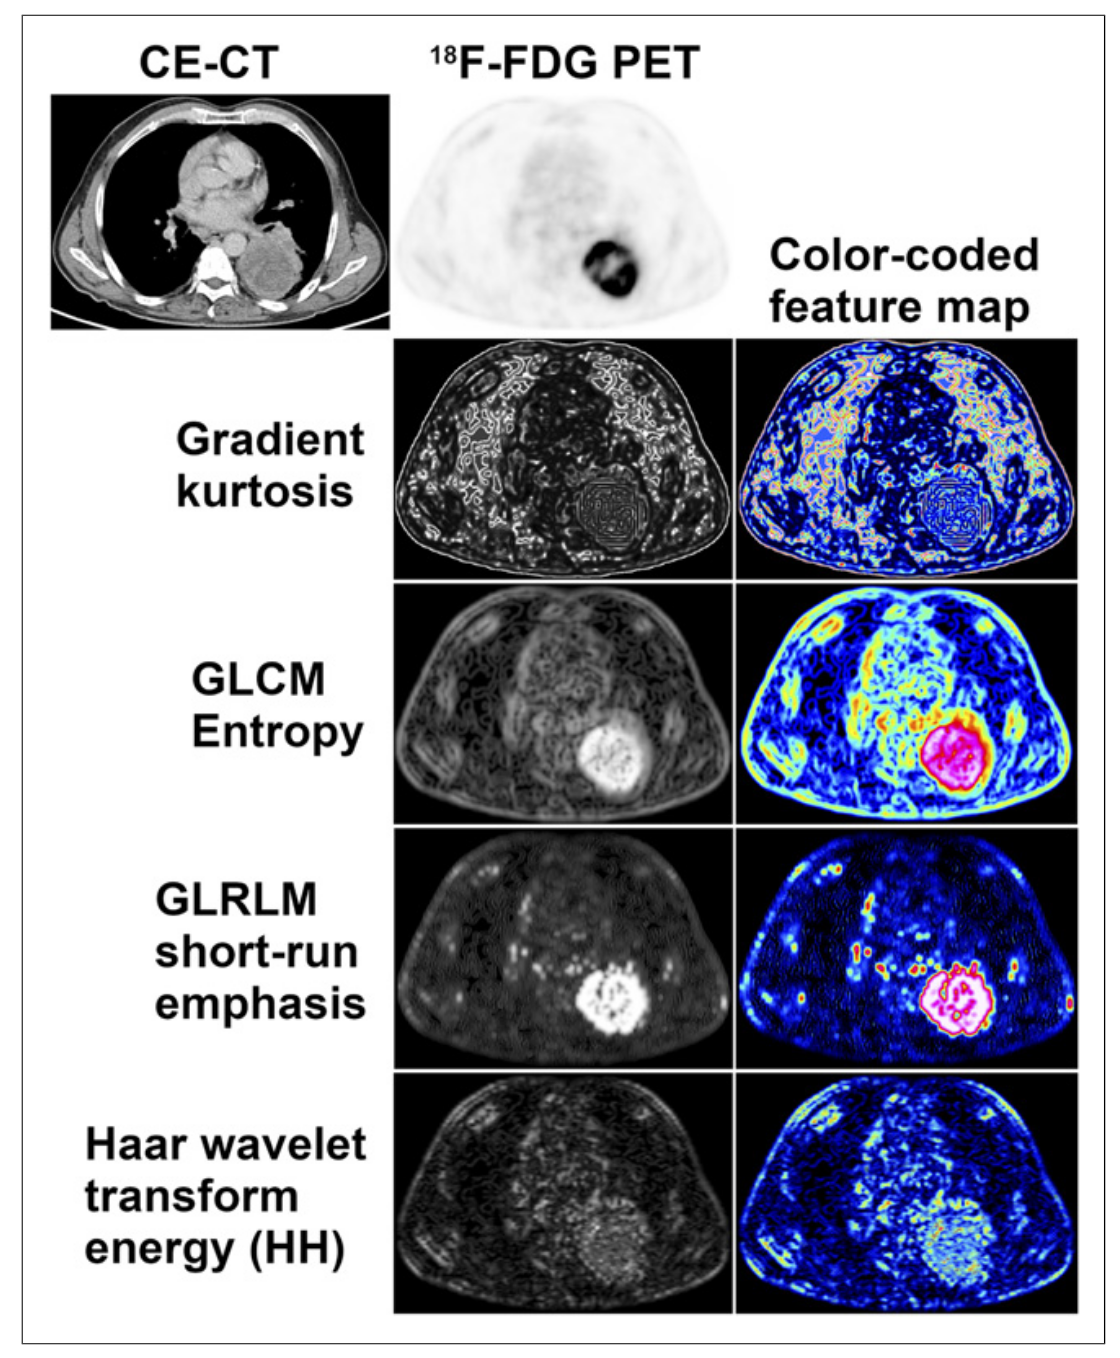
\includegraphics[width=0.6\textwidth]{figures/fig001.png}
    \caption*{Autor: \cite{mayerhoeferIntroductionRadiomics2020}}
    \label{fig:fig001}
\end{figure}

 A matriz de coocorrência de níveis de cinza, do termo \gls{glcm}, é um histograma em níveis de cinza de segunda ordem. O GLCM captura relações espaciais entre pares de \textit{pixels} ou \textit{voxels} com níveis de cinza pré-definidos, em diferentes direções (horizontal, vertical ou diagonal para análise 2D, 13 direções para 3D) e com uma distância pré-definida entre os \textit{pixels} ou \textit{voxels}. As características de GLCM incluem entropia, uma medida composta pela medida da inomogeneidade ou aleatoriedade dos níveis de cinza, momento angular de segunda ordem (também chamado de uniformidade ou energia), que reflete a homogeneidade ou ordem dos níveis de cinza e contraste, que enfatiza as diferenças nos níveis de cinza entre \textit{pixels} ou \textit{voxels} pertencentes a um par de \textit{pixel} ou \textit{voxel}. A Figura \ref{fig:fig002} ilustra um matriz que atua como um contador dos pares de \textit{pixel} ou \textit{voxel}.

 A matriz de comprimento de corrida de níveis de cinza, do termo 
 \textit{Gray-Level Run-length Matrix} (GLRLM), fornece informações sobre a distribuição espacial das sequências de \textit{pixels} consecutivos com os mesmos níveis de cinza, em uma ou mais direções, em 2 ou 3 dimensões. As características da GLRLM incluem fração, que avalia a porcentagem de \textit{pixels} ou \textit{voxels} dentro da região de interesse que fazem parte das sequências e, portanto, reflete a granulosidade. 

A matriz de zona do tamanho dos níveis de cinza, do termo \textit{Gray-Level Size Zone Matrix} (GLSZM), é baseada no mesmo princípio do GLRLM porém aqui, contagens do número de grupos (chamados zonas) de \textit{pixels} ou \textit{voxels} vizinhos interconectados com o mesmo nível de cinza formam a base para a matriz, como visto na Figura \ref{fig:fig002}. Uma textura mais homogênea resultará em uma matriz mais ampla e plana. A GLSZM não é calculada para diferentes direções, mas pode ser calculada para diferentes distâncias de \textit{pixels} ou \textit{voxels} que definem a vizinhança. As características da GLSZM podem ser calculadas em 2 dimensões (8 \textit{pixels} vizinhos) ou 3 dimensões (26 \textit{voxels} vizinhos) e, seguindo as definições da GLRLM, incluem fração (porcentagem de \textit{pixels} ou \textit{voxels} que fazem parte das zonas), ênfase em zonas pequenas e grandes, entre outras.

\begin{figure}[htbp]
    \centering
    \caption{Aplicação de Vizinhos em Abordagens Radiômicas}
    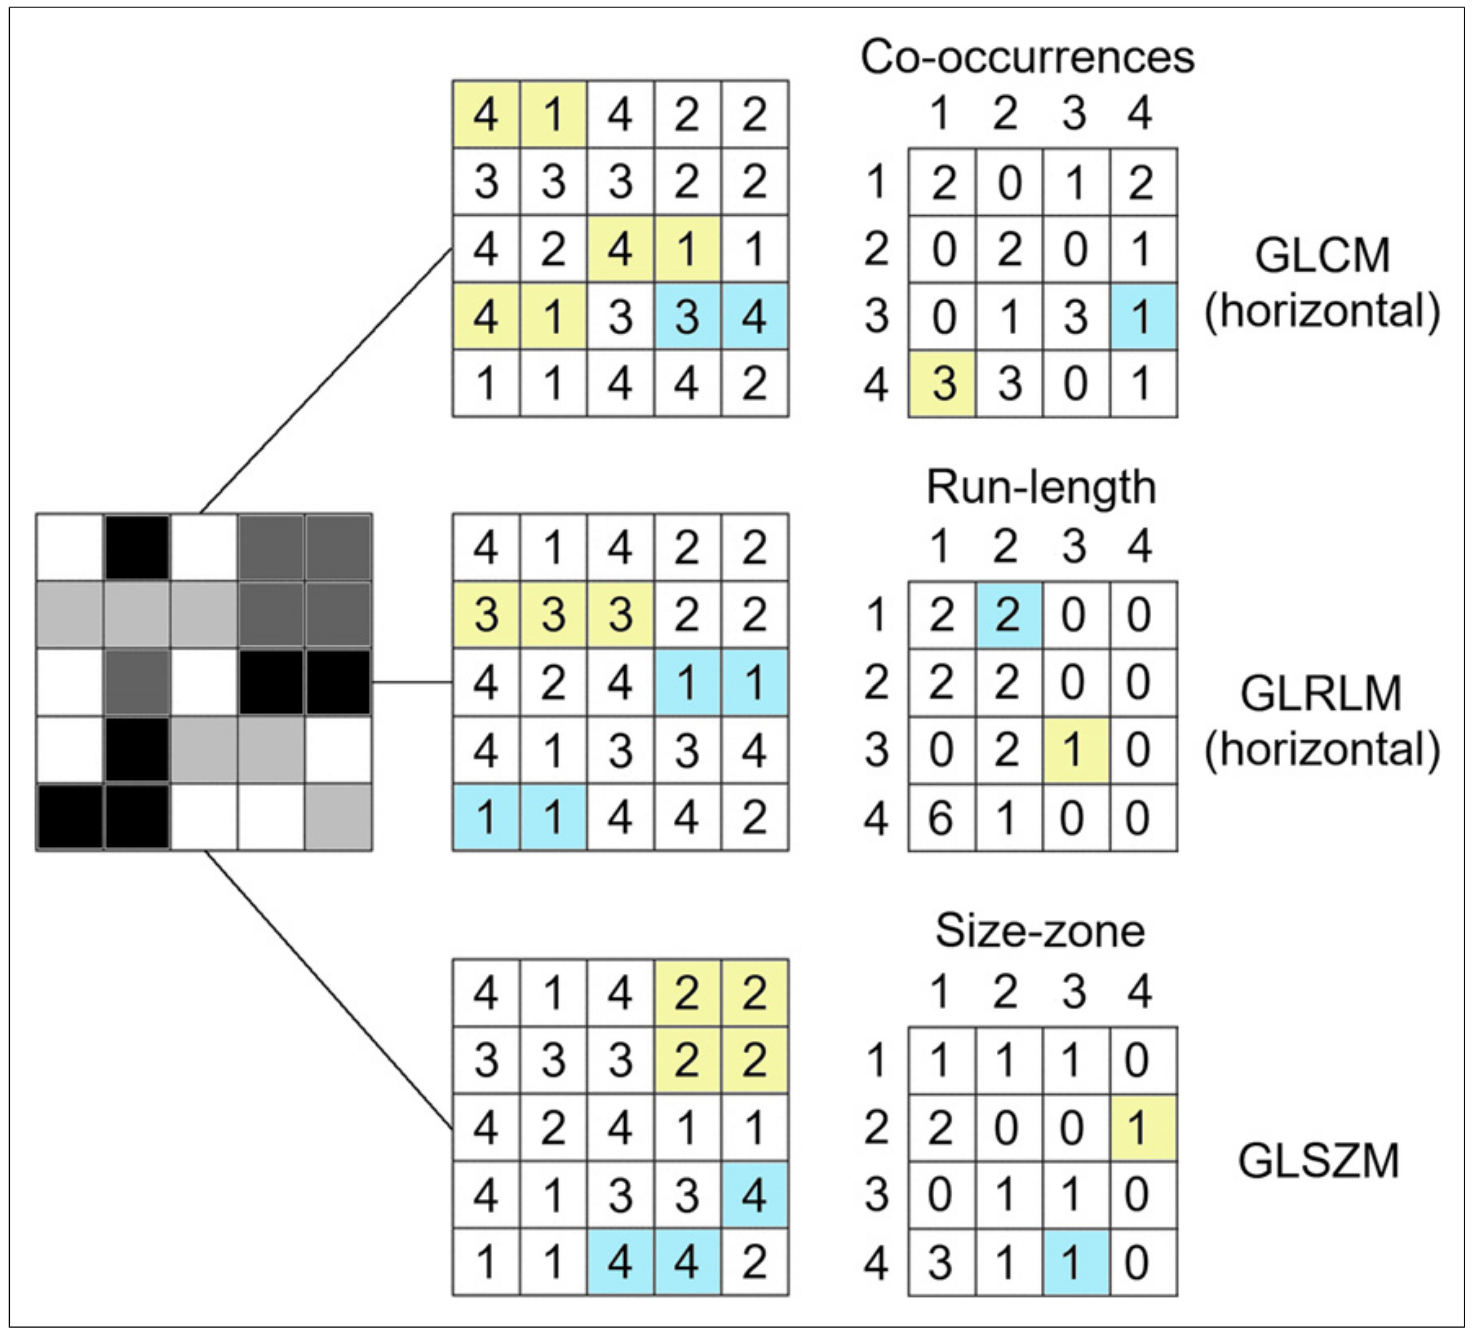
\includegraphics[width=0.6\textwidth]{figures/fig002.png}
    \caption*{Autor: \cite{mayerhoeferIntroductionRadiomics2020}}
    \label{fig:fig002}
\end{figure}

%--------------------------------------------------------
\subsection{Características de Modelo}

As análises baseadas em modelos visam interpretar características em níveis de cinza espaciais para caracterizar objetos ou formas. Um modelo parametrizado de geração de textura é calculado e ajustado à região de interesse, do termo \gls{roi}, e seus parâmetros estimados são utilizados como características radiômicas. O modelo autorregressivo é um exemplo de abordagem baseada em modelo e baseia-se na ideia de que o nível de cinza de um \textit{pixel} é uma soma ponderada dos níveis de cinza de 4 \textit{pixels} vizinhos. Além disso, o $\sigma$, o qual carrega informações sobre a variância do erro de previsão mínimo, mede a regularidade da textura. A análise fractal também produz recursos que podem ser usados na análise radiômica, em particular a dimensão fractal, que reflete a taxa de adição de detalhe estrutural com o aumento da magnificação, escala ou resolução e, portanto, serve como uma medida de complexidade. A lacunaridade, um recurso que mede a falta de invariância rotacional ou translacional, reflete a inomogeneidade \cite{mayerhoeferIntroductionRadiomics2020}.

%--------------------------------------------------------
\subsection{Características de Transformação}
Métodos baseados em transformadas, incluindo transformadas de \textit{Fourier}, \textit{Gabor} e de \textit{wavelets} de \textit{Haar}, analisam padrões de níveis de cinza em um espaço diferente. A transformada discreta \textit{wavelet} de \textit{Haar}, por exemplo, analisa o conteúdo da frequência de uma imagem em diferentes escalas. A decomposição por \textit{wavelets} de uma imagem é possível aplicando um par de filtros espelhados em quadratura, um filtro de passa-alta e um de passa-baixa. Embora o filtro de passa-alta destaque as mudanças no nível de cinza e, assim, enfatize detalhes da imagem, o filtro de passa-baixa suaviza a imagem em termos de nível de cinza, removendo detalhes da imagem. Após a decomposição do sinal, um conjunto de canais de frequência orientados espacialmente está disponível, o qual é usado para descrever a variabilidade local da imagem. As energias dentro dos canais de frequência são então usadas como características. A filtragem de passa-alta em ambas as direções, parte inferior da Figura \ref{fig:fig001}, captura detalhes diagonais, a filtragem de passa-alta seguida por filtragem de passa-baixa captura bordas verticais, a filtragem de passa-baixa seguida da filtragem de passa-alta captura bordas horizontais, e a filtragem de passa-baixa em ambas as direções captura as frequências mais baixas, em diferentes escalas. Notavelmente, a transformação por \textit{wavelets} pode ser usada não apenas para a geração de características radiômicas, mas também para segmentação de imagens ou como um passo de pré-processamento para análise de textura \cite{mayerhoeferIntroductionRadiomics2020}.

%---------------------------------------------------------
\section{REDES NEURAIS CONVOLUCIONAIS}
\label{sec:cnn}


Os autores \citeonline{lecunHandwrittenDigitRecognition1989} pesquisaram sobre o reconhecimento de caracteres em documentos escritos à mão, criando a arquitetura LeNet, uma rede que consiste em camadas convolucionais seguidas por camadas de \textit{pooling}, e finalizando com camadas totalmente conectadas. Os autores introduziram o \textit{backpropagation} a redes convolucionais, permitindo o aprendizado automático e substituindo o uso de técnicas para escolha manual de coeficientes. \citeonline{lecunHandwrittenDigitRecognition1989}, ainda estudando a classificação de caracteres, expandem a LeNet para a LeNet-5, uma rede que firmou a superioridade das redes convolucionais na tarefa de classificação de imagens se comparado a outros métodos da época.

Como o nome sugere, a camada convolucional desempenha um papel vital no funcionamento da \gls{cnn}. Os parâmetros das camadas concentram-se no uso de \textit{kernels} treináveis. Esses \textit{kernels} geralmente são pequenos em dimensionalidade espacial, mas se estendem por toda a profundidade da entrada. Quando os dados passam por uma camada convolucional, ela aplica cada filtro na dimensionalidade espacial da entrada para produzir um mapa de ativação 2D. À medida que se percorre a entrada, o produto escalar é calculado para cada valor nesse \textit{kernel}. A partir disso, a rede aprenderá \textit{kernels} que ``disparam'' quando detectam uma característica específica em uma determinada posição espacial da entrada. Esses são comumente conhecidos como ativações conforme descrito na Figura \ref{fig:fig024}.

\begin{figure}[h!]
    \centering
    \caption{Representação visual da camada convolucional. O elemento central do \textit{kernel} é aplica no vetor de entrada, que é calculado e substituído pela ponderada dele mesmo e de quaisquer pixels próximos.}
    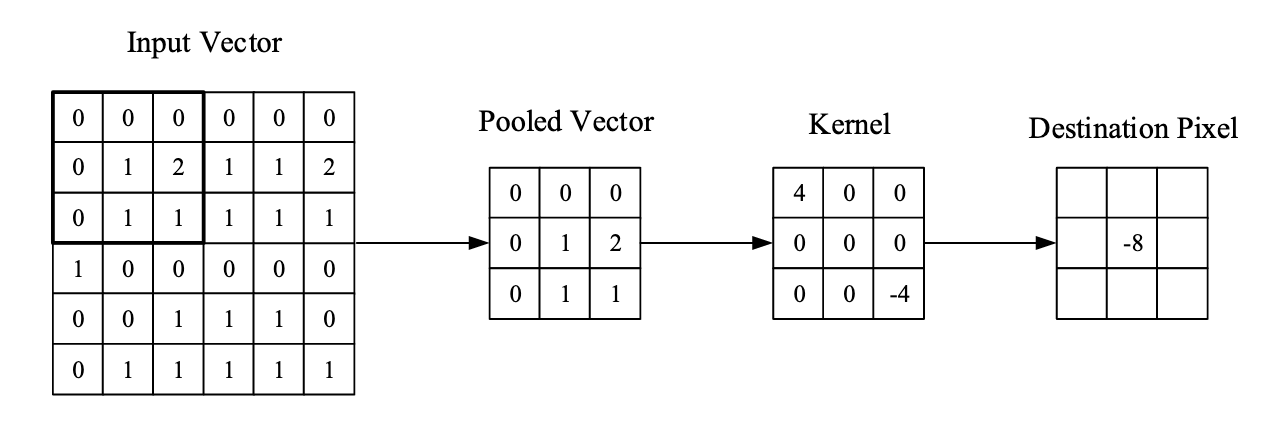
\includegraphics[width=0.6\textwidth]{figures/fig024.png}
    \caption*{Fonte: \cite{osheaIntroductionConvolutionalNeural2015c}}
    \label{fig:fig024}
\end{figure}

Cada \textit{kernel} terá um mapa de ativação correspondente, que será empilhado ao longo da dimensão de profundidade para formar o volume completo de saída da camada convolucional. Como mencionado anteriormente, treinar redes neurais artificiais tendo imagens como entrada resulta em modelos demasiadamente grandes para serem treinados de forma eficaz. Isso ocorre devido à conexão totalmente densa dos neurônios padrão das redes neurais artificiais. Para mitigar esse problema, cada neurônio em uma camada convolucional é conectado apenas a uma pequena região do volume de entrada \cite{osheaIntroductionConvolutionalNeural2015c}. 

A dimensionalidade dessa região é comumente chamada de ``tamanho do campo receptivo'' do neurônio. A magnitude da conectividade ao longo da profundidade geralmente é igual à profundidade da entrada. Por exemplo, se a entrada para a rede for uma imagem de tamanho 64x64x3 (uma imagem colorida RGB com dimensionalidade de 64x64) e for definido o tamanho do campo receptivo como 6x6, é obtido um total de 108 pesos em cada neurônio dentro da camada convolucional (6x6x3, onde 3 é a magnitude da conectividade na profundidade do volume). Para colocar isso em perspectiva, um neurônio padrão visto em outras formas de redes neurais artificiais conteria $12.288$ pesos cada. 

Camadas convolucionais também conseguem reduzir significativamente a complexidade do modelo por meio da otimização de sua saída. Essas otimizações são feitas por meio de três hiperparâmetros: profundidade, \textit{stride} e \textit{zero-padding}. 

A profundidade do volume de saída produzido pelas camadas convolucionais pode ser definida manualmente através do número de neurônios dentro da camada para uma mesma região da entrada. Isso pode ser observado em outras formas de redes neurais artificiais, onde todos os neurônios da camada oculta estão diretamente conectados a cada neurônio anterior. Reduzir esse hiperparâmetro pode minimizar significativamente o número total de neurônios da rede, mas também pode reduzir as capacidades de reconhecimento de padrões do modelo. 

Também é possível definir o \textit{stride}, que determina como é configurada a profundidade em torno da dimensionalidade espacial da entrada para posicionar o campo receptivo. Por exemplo, se o \textit{stride} for definido como 1, obtém-se um campo receptivo fortemente sobreposto, produzindo ativações extremamente grandes. Por outro lado, ao configurar o \textit{stride} para um número maior reduz a sobreposição e gera uma saída com dimensões espaciais menores.  

O \textit{zero-padding} é o processo de adicionar bordas à entrada, sendo um método eficaz para proporcionar maior controle sobre a dimensionalidade dos volumes de saída. É importante entender que, ao se usar dessas técnicas, a dimensionalidade espacial da saída das camadas convolucionais é alterada. Para este cálculo pode-se usar a seguinte Equação \ref{eq:cnn_output}.

\begin{equation}
\frac{(V - R) + 2Z}{S + 1}
\label{eq:cnn_output}
\end{equation}

O termo $V$ representa o tamanho do volume de entrada (altura x largura x profundidade), $R$ representa o tamanho do campo receptivo, $Z$ é a quantidade de \textit{zero-padding} definida e $S$ refere-se ao \textit{stride}. Se o resultado calculado a partir desta equação não for um número inteiro, o \textit{stride} foi configurado incorretamente, pois os neurônios não conseguirão se ajustar perfeitamente à entrada \cite{osheaIntroductionConvolutionalNeural2015c}.

%---------------------------------------------------------
\section{RESNET}
\label{sec:resnet}

A \textit{ResNet} (Rede Residual) é uma arquitetura de rede neural profunda amplamente utilizada em tarefas de visão computacional, como classificação de imagens, detecção de objetos e segmentação de imagens. Ela foi introduzida por \citeonline{heDeepResidualLearning2015}, e se destacou por ganhar a competição \textit{ImageNet} em 2015 com uma precisão significativamente maior do que as arquiteturas anteriores. A principal característica da \textit{ResNet} é sua capacidade de treinar redes muito profundas sem sofrer com o problema do ``desvanecimento do gradiente'' que afeta principalmente redes neurais profundas e impede o treinamento de progredir por conta de valores muito baixos de gradiente, problema este muito comum em redes tradicionais muito profundas. A \textit{ResNet} introduz um conceito chave chamado bloco residual que é um componente da rede onde a entrada do bloco é somada à sua saída antes de passar para a próxima camada. Esta conexão direta é chamada de conexão de salto e pode ser observada na Figura \ref{fig:fig013}.

\begin{figure}[h!]
    \centering
    \caption{Conexão de Salto}
    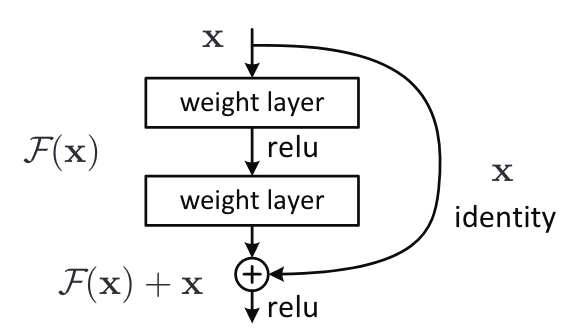
\includegraphics[width=0.6\textwidth]{figures/fig013.png}
    \caption*{Fonte: \cite{aiSelfAttentionBasedFusion2023}}
    \label{fig:fig013}
\end{figure}

A ResNet é composta por vários blocos residuais empilhados.
Existem várias versões da \textit{ResNet}, como \textit{ResNet}-18, \textit{ResNet}-34, \textit{ResNet}-50, \textit{ResNet}-101, e \textit{ResNet}-152, onde os números indicam a profundidade total da rede, ou seja, o número de camadas.

%--------------------------------------------------------
\subsection{Extração de Características Profundas}
\label{subsec:extract_features}

Para extrair características profundas das imagens de \gls{rmc}, foi empregada a arquitetura pré-treinada de uma rede \textit{ResNet50}. As redes \textit{ResNet50} ficaram muito conhecidas em meados do ano de 2015 por vencer diversas competições em visão computacional, incluindo o primeiro lugar na competição de classificação de imagens \textit{ILSVRC} 2015. As redes \textit{ResNet}, do termo \textit{Residual Networks}, inovaram em sua época trazendo uma nova forma de treinar modelos que possuem maior profundidade, chegando a mais de 100 camadas, com resultados superiores à outros modelos convolucionais competitivos, como o \textit{VGG19}, sem sofrer sintomas comuns a redes neurais muito profundas como o \textit{overfitting} e a saturação ou a ausência dos gradientes em tempo de treino. Os autores da \textit{ResNet} sugeriram o uso de saltos de conexão entre as camadas da rede afim de manter os gradientes relevantes e controlados entre uma camada e outra.  A \textit{ResNet50} é um modelo de rede neural convolucional profunda de $50$ camadas que compreende muitos blocos residuais. A cada bloco, se encontram módulos de convolução e uma conexão de salto que transfere a informação do bloco anterior para o próximo bloco. A conexão de salto ajuda a reter a informação semântica mais baixa aprendida nas camadas anteriores, que de outra forma se tornaria abstrata devido à conexão de longa cadeia. A conexão de salto também evita que o gradiente desapareça nas camadas mais profundas, fornecendo um caminho alternativo para a retropropagação. A informação da conexão de salto é adicionada à informação calculada em cada bloco \cite{heDeepResidualLearning2015}.

Várias abordagens de sucesso aplicaram redes convolucionais para extrair características genéricas para tarefas de recuperação de imagens e obtiveram resultados promissores. Elas utilizam principalmente o poder das características locais para gerar uma representação de uma imagem genérica baseada em redes convolucionais pré-treinadas. As representações das camadas finais da rede convolucional são utilizadas para capturar características semânticas para o fim de nível de categoria à classificação que o modelo se dispõe \cite{alzubiContentbasedImageRetrieval2017b}.

%---------------------------------------------------------
\section{REDE SQUEEZE AND EXCITATION}
\label{sec:se_net}

Para cada camada convolucional, um conjunto de filtros é aprendido para expressar padrões de conectividade espacial local ao longo dos canais de entrada. Em outras palavras, espera-se que os filtros convolucionais sejam combinações informativas ao fundir informações espaciais e baseadas nos canais dentro de campos receptivos locais.
Ao empilhar uma série de camadas convolucionais intercaladas com não linearidades e redução de amostragem, as \gls{cnn}s são capazes de capturar padrões hierárquicos com campos receptivos globais, funcionando como descrições de imagem poderosas \cite{huSqueezeandExcitationNetworks2018}. 

Estudos de \citeonline{huSqueezeandExcitationNetworks2018}, demonstraram que o desempenho das redes pode ser aprimorado ao incorporar explicitamente mecanismos de aprendizado que ajudam a capturar correlações espaciais, sem a necessidade de supervisão adicional. Neste sentido, foi proposto um mecanismo que permite à rede realizar a recalibração de características, por meio do qual ela pode aprender a usar informações globais para enfatizar seletivamente características informativas e suprimir aquelas menos úteis. Este estudo intitulado \gls{se} Net, investiga um aspecto diferente no design arquitetural, a relação entre canais ao introduzir o bloco \gls{se}.

Os blocos \gls{se} podem ser construídos para qualquer transformação conforme a indica a Equação \ref{eq:se_transform} onde $\mathbf{U}$ representa a saída da transformação inicial da rede neural, antes da aplicação do bloco \gls{se}.

\begin{equation}
\mathcal{F}_{tr} : \mathbf{X} \rightarrow \mathbf{U}, \mathbf{X} \in R^{H' \times W' \times C'}, \mathbf{U} \in R^{H \times W \times C}
\label{eq:se_transform}
\end{equation}

Sendo $\mathbf{V} = [\mathbf{v}_1, \mathbf{v}_2, \ldots, \mathbf{v}_C]$ os filtros de aprendidos onde $\mathbf{v}_C$ se refere ao parâmetro de $c$-ésimo filtro. As saídas das convoluções podem ser escritas da seguinte forma: $\mathcal{F}_{tr} \mathbf{U} = [\mathbf{u}_1, \mathbf{u}_2, \ldots, \mathbf{u}_C]$, sendo o termo $\mathbf{u}_C$ descrito na equação \ref{eq:se}. 

\begin{equation}
\mathbf{u}_c = \mathbf{v}_c \ast \mathbf{X} = \sum_{s=1}^{C'} \mathbf{v}_c^s \ast \mathbf{x}^s
\label{eq:se}
\end{equation}

O termo $\ast$ denota convolução, $\mathbf{v}_c$ é um filtro espacial 2D e representa um único canal de $\mathbf{v}_c$ que atua no canal correspondente de $\mathbf{X}$. 
Tendo como o objeto garantir que a rede seja capaz de aumentar sua sensibilidade a características informativas, para que possam ser exploradas por transformações subsequentes, e suprimir as menos úteis. Foi proposto um modelo explícito das interdependências de canal para recalibrar as respostas dos filtros em duas etapas — \textit{squeeze} e \textit{excitation} —, antes de serem alimentadas na transformação subsequente. Um diagrama de um bloco de construção \gls{se} é demonstrado na Figura \ref{fig:fig025}.

\begin{figure}[h!]
    \caption{Fluxo do Bloco SE - Após blocos convolucionais normais, uma cama da de \textit{squeeze} seguida e uma camada de \textit{excitation} é aplicada e por fim os valores originais são escalonados pelo resultado.}
    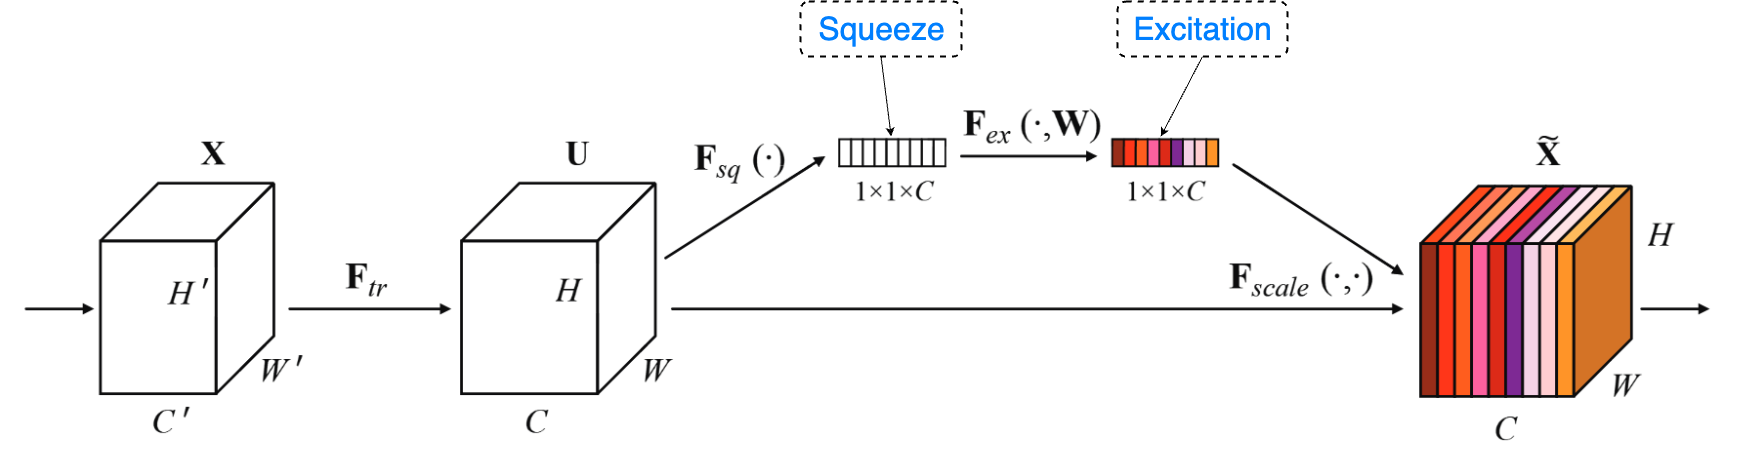
\includegraphics[height=0.27\textwidth]{figures/fig025.png}
    \caption*{Fonte: Adaptado de \cite{huSqueezeandExcitationNetworks2018}}
    \label{fig:fig025}
\end{figure}


%---------------------------------------------------------
\subsection{Squeeze: Informação Global}
\label{subsec:squeeze}

Para lidar com o problema de explorar as dependências entre os canais, é considerado o primeiro sinal de cada canal nas características de saída. Cada um dos filtros aprendidos opera com um campo receptivo local e, consequentemente, cada unidade da saída da transformação $\mathbf{U}$ é incapaz de explorar informações contextuais fora dessa região. Esse problema se torna ainda mais grave nas camadas mais baixas da rede, cujos campos receptivos são menores.

Para mitigar esse problema, foi proposto comprimir as informações espaciais globais em um descritor de canal. Isso é obtido por meio de uma instrução de \textit{average pooling} global para gerar estatísticas específicas de cada canal. O cálculo do \textit{average pooling} pode ser conferido na Equação \ref{eq:avgpool}.

\begin{equation}
z_c = \mathbf{F}_{sq}(\mathbf{u}_c) = \frac{1}{H \times W} \sum_{i=1}^{H} \sum_{j=1}^{W} u_c(i, j)
\label{eq:avgpool}
\end{equation}

%---------------------------------------------------------
\subsection{Excitation: Recalibração Adaptativa}
\label{subsec:excitation}

Para aproveitar as informações agregadas na operação de \textit{squeeze}, uma segunda operação que tem como objetivo capturar completamente as dependências entre os canais. Para cumprir esse objetivo, a função deve atender a dois critérios: primeiro, ela precisa ser flexível (em particular, deve ser capaz de aprender uma interação não linear entre os canais) e, segundo, ela deve aprender uma relação não mutuamente exclusiva, pois é de interesse garantir que vários canais possam ser enfatizados, em vez de apenas uma ativação \textit{one-hot}. Para atender a esses critérios, emprega-se um mecanismo de \textit{gating} simples com uma ativação sigmoide conforme demonstrado na Equação \ref{eq:excitation}:

\begin{equation}
\mathbf{s} = \mathbf{F}_{ex}(\mathbf{z}, \mathbf{W}) = \sigma(g(\mathbf{z}, \mathbf{W})) = \sigma(\mathbf{W}_2 \delta(\mathbf{W}_1 \mathbf{z}))
\label{eq:excitation}
\end{equation}

\noindent sendo que o termo $\delta$ se refere à função de ativação ReLU \cite{nairRectifiedLinearUnits}, $W_1 \in \mathbb{R}^{\frac{C}{r} \times C}$ e $W_2 \in \mathbb{R}^{C \times \frac{C}{r}}$. Para limitar a complexidade do modelo e auxiliar na generalização, o mecanismo de \textit{gating} é parametrizado formando um gargalo com duas camadas totalmente conectadas ao redor da não linearidade, ou seja, uma camada de redução de dimensionalidade com os parâmetros $W_1$ e razão de redução $r$, seguida de uma ReLU e, em seguida, uma camada de aumento de dimensionalidade com os parâmetros $W_2$. A saída final do bloco é obtida ao redimensionar a saída da transformação $U$ com as ativações conforme Equação \ref{eq:se_scale}.

\begin{equation}
\tilde{\mathbf{x}}_c = \mathbf{F}_{scale}(\mathbf{u}_c, s_c) = s_c \cdot \mathbf{u}_c 
\label{eq:se_scale}
\end{equation}

\noindent onde $\tilde{\mathbf{X}} = [\tilde{\mathbf{x}}_1, \tilde{\mathbf{x}}_2, \dots, \tilde{\mathbf{x}}_C]$ e $\mathbf{F}_{scale}(\mathbf{u}_c, s_c)$ se referem a multiplicação no nível dos canais entre os mapas de características $\mathbf{u}_c \in \mathbb{R}^{H \times W}$ e o valor escalar $s_c$.

%---------------------------------------------------------
\subsection{Utilização em redes conhecidas: SE-Resnet}
\label{subsec:util_resnet}

A flexibilidade do bloco \gls{se} significa que ele pode ser aplicado diretamente a transformações além das convoluções padrão. Para ilustrar esse ponto, os autores desenvolveram as redes \gls{se}  integrando blocos \gls{se} em arquiteturas modernas com \textit{designs} sofisticados. A Figura \ref{fig:fig026} demonstra o esquema de um módulo SE-ResNet. Nele, a transformação do bloco \gls{se}, $F_{tr}$, é considerada o ramo não identidade de um módulo residual. As operações de \textit{squeeze} e \textit{excitation} atuam antes da soma com o ramo identidade.


\begin{figure}[h!]
    \centering
    \caption{Módulo SE-Resnet}
    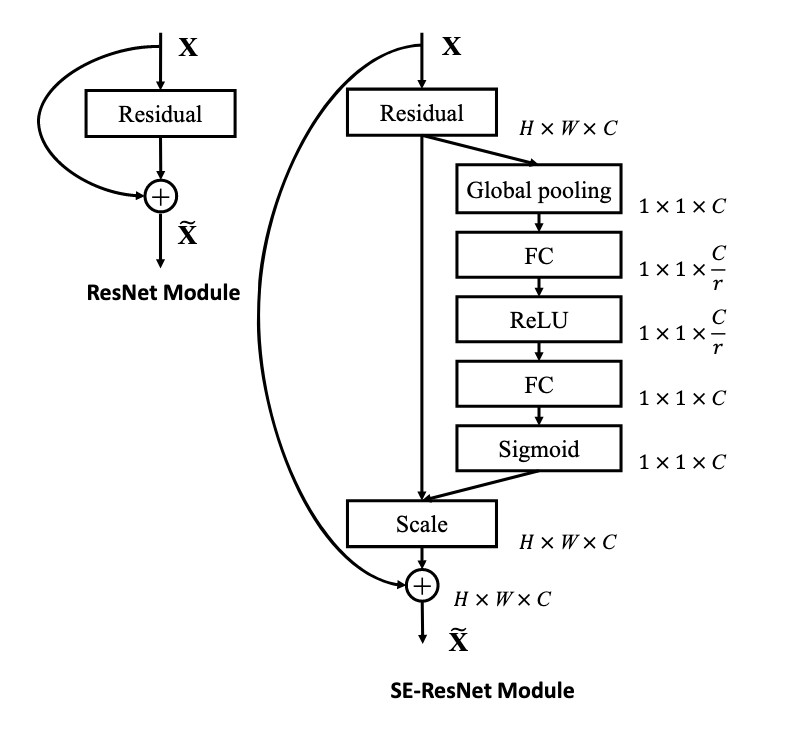
\includegraphics[width=0.6\textwidth]{figures/fig026.png}
    \caption*{Fonte: Adaptado de \cite{huSqueezeandExcitationNetworks2018}}
    \label{fig:fig026}
\end{figure}

Para que o bloco SE proposto seja viável na prática, ele deve fornecer um equilíbrio eficaz entre a complexidade do modelo e o desempenho, o que é importante para escalabilidade. Foi definida uma razão de redução $r$ como 16 em todos os experimentos, exceto onde indicado de outra forma. 

O valor $r$ é um hiperparâmetro importante pois permite variar a capacidade e o custo computacional dos blocos \gls{se} no modelo. O autor do trabalho conduz experimentos baseados no SE-ResNet-50 para uma variedade de valores diferentes de $r$. A comparação vista na Figura  \ref{fig:fig027}, revela que o desempenho não melhora monotonicamente com o aumento da capacidade. Isso provavelmente é resultado do bloco SE ajustar em excesso as interdependências de canal do conjunto de treinamento. Definir $r = 16$ alcançou um bom equilíbrio entre precisão e complexidade e, consequentemente, foi o valor utilizado pelos autores nos experimentos. O Algoritmo \ref{alg:se_block} reflete a implementação do bloco \gls{se}.

\begin{figure}[h!]
    \centering
    \caption{Conjunto de Validação Aplicado na SE-ResNet-50}
    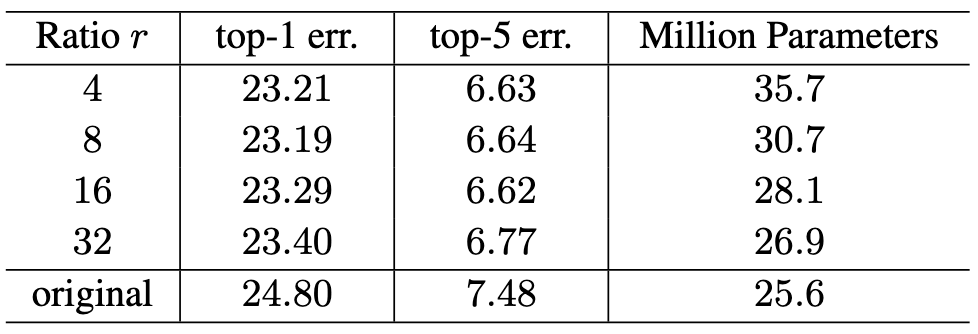
\includegraphics[width=0.6\textwidth]{figures/fig027.png}
    \caption*{Fonte: Adaptado de \cite{huSqueezeandExcitationNetworks2018}}
    \label{fig:fig027}
\end{figure}

% ----------------- ALGORITMO SQUEEZE AND EXCITATION NET ------------------
\begin{algorithm}
\caption{Bloco Squeeze-and-Excitation (SE)}
\label{alg:se_block}
\textbf{Entrada:} Mapa de características $\mathbf{U} \in \mathbb{R}^{H \times W \times C}$\\
\textbf{Saída:} Mapa de características recalibrado $\tilde{\mathbf{U}} \in \mathbb{R}^{H \times W \times C}$
\begin{algorithmic}[1]
\STATE \textbf{Squeeze:} Executa o \textit{average pooling} global para agregar as dimensões espaciais:
\[
z_c = \frac{1}{H \times W} \sum_{i=1}^H \sum_{j=1}^W u_c(i, j), \quad \forall c \in \{1, \dots, C\}
\]
\STATE \textbf{Excitation:} Usa duas camadas totalmente conectadas para modelar a interdependência dos canais:
\[
\mathbf{s} = \sigma(\mathbf{W}_2 \delta(\mathbf{W}_1 \mathbf{z}))
\]
onde:
\begin{itemize}
    \item $\mathbf{W}_1 \in \mathbb{R}^{\frac{C}{r} \times C}$: Camada de redução de dimensionalidade
    \item $\mathbf{W}_2 \in \mathbb{R}^{C \times \frac{C}{r}}$: Camada de restauração da dimensão original
    \item $\delta$: Ativação ReLU
    \item $\sigma$: Ativação Sigmoide
\end{itemize}
\STATE \textbf{Reescala:} Recalibra o mapa de características usando as ativações:
\[
\tilde{\mathbf{u}}_c = s_c \cdot \mathbf{u}_c, \quad \forall c \in \{1, \dots, C\}
\]
\RETURN $\tilde{\mathbf{U}} = [\tilde{\mathbf{u}}_1, \tilde{\mathbf{u}}_2, \dots, \tilde{\mathbf{u}}_C]$
\end{algorithmic}
% \caption*{Fonte: Autor}
\end{algorithm}


%--------------------------------------------------------
\section{ARQUITETURA TRANSFORMERS}
\label{sec:transformers}

Os \textit{transformers} consistem em uma arquitetura que possui como um de seus propósitos resolver as limitações das arquiteturas recorrentes e sua dificuldade em manter as relações entre pontos dentre as camadas recorrentes além das restrições vinculadas ao custo de computação sequencial. O modelo de arquitetura \textit{transformers} se utiliza do mecanismo de atenção e este se tornou parte essencial de modelos eficazes de modelagem e transdução de sequências em diversas tarefas, permitindo a modelagem de dependências sem considerar a distância entre elas nas sequências de entrada ou saída. Os \textit{transformers} como arquitetura descarta o uso de módulos de recorrência e se utiliza inteiramente do mecanismo de atenção para capturar as dependências globais entre entrada e saída. Os \textit{transformers} também são responsáveis por um ganho significante em paralelismo em sua execução \cite{vaswaniAttentionAllYou2023}.

\begin{figure}[htbp]
    \centering
    \caption{Arquitetura \textit{Transformers}}
    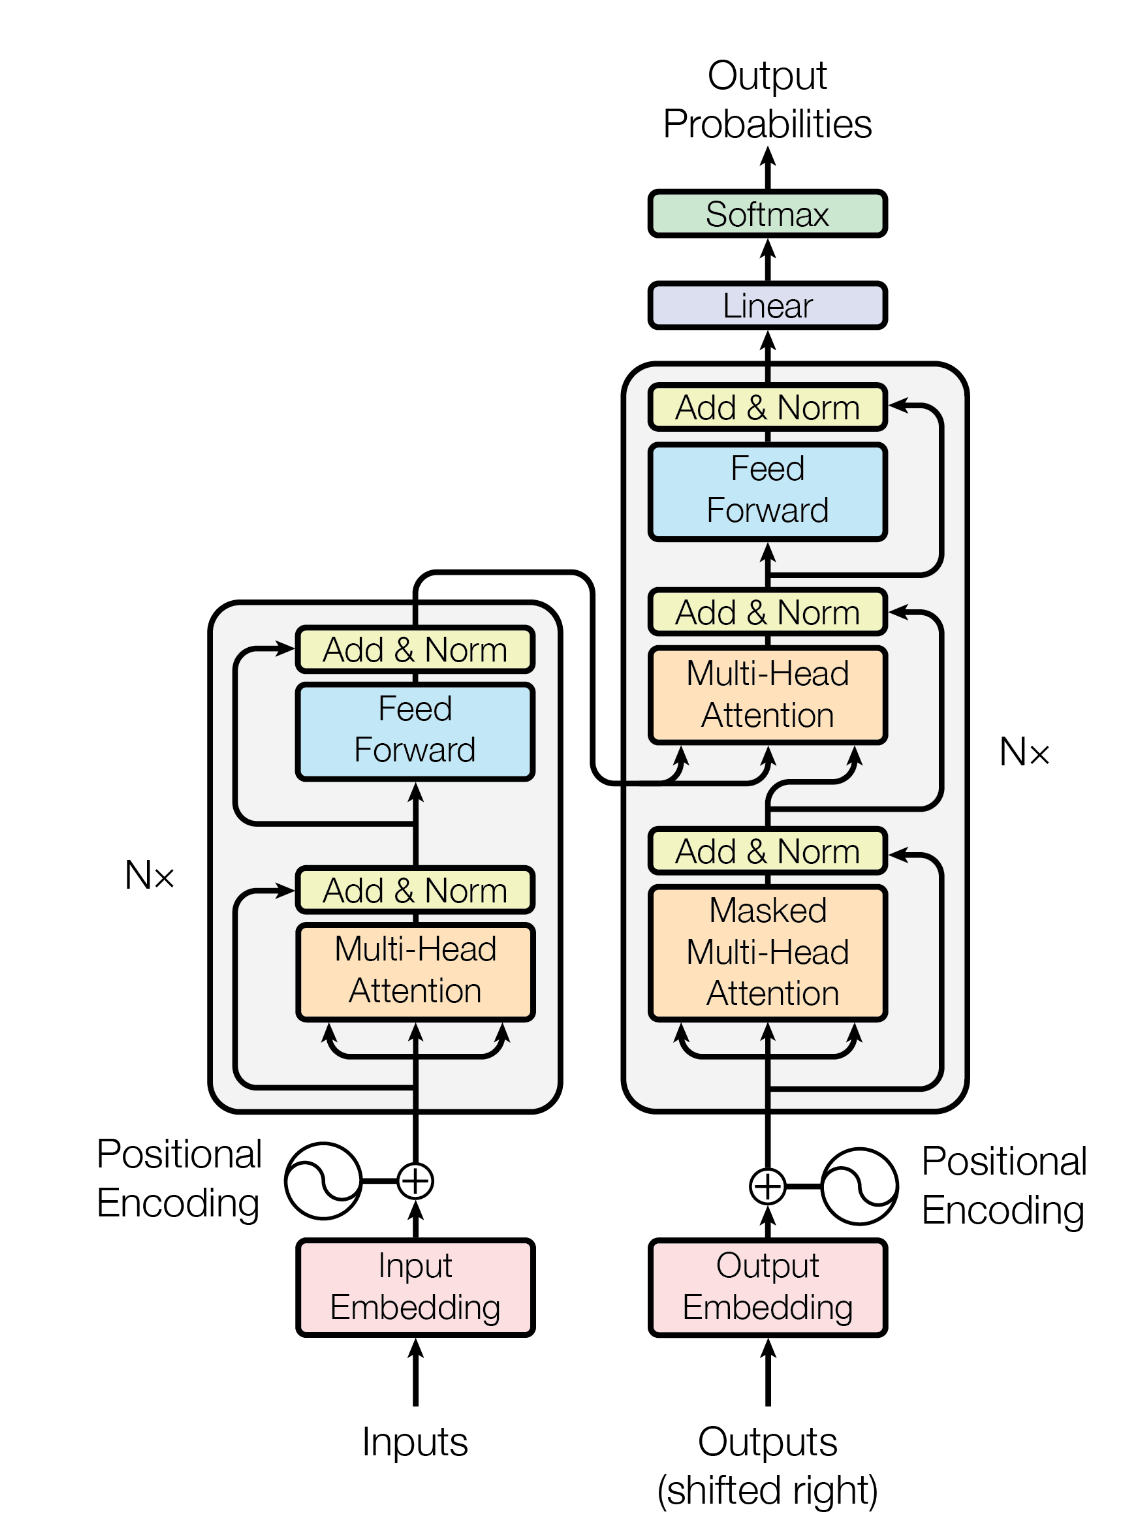
\includegraphics[scale=0.6]{figures/fig004.png}
    \caption*{Autor: \citeonline{vaswaniAttentionAllYou2023}}
    \label{fig:fig004}
\end{figure}

Os \textit{transformers} são compostos por um \textit{Encoder} e um \textit{Decoder}, representados pelos os blocos da esquerda e direita respectivamente apresentados na Figura \ref{fig:fig004}. Em ambos \textit{Encoder} e \textit{Decoder}, tem-se como bloco cerne da rede intitulado de atenção multi-cabeças. O mecanismo de atenção pode ser descrito mapeando uma \textit{query} a um par de chave e valor, onde a \textit{query}, a chave e o valor são todos vetores de saída. A saída é computada como uma soma ponderada dos valores onde o peso destinado a cada valor é computado por uma função de compatibilidade da \textit{query} com a chave correspondente.

\begin{figure}[htbp]
    \centering
    \caption{Módulo de Atenção Multi-Cabeças}
    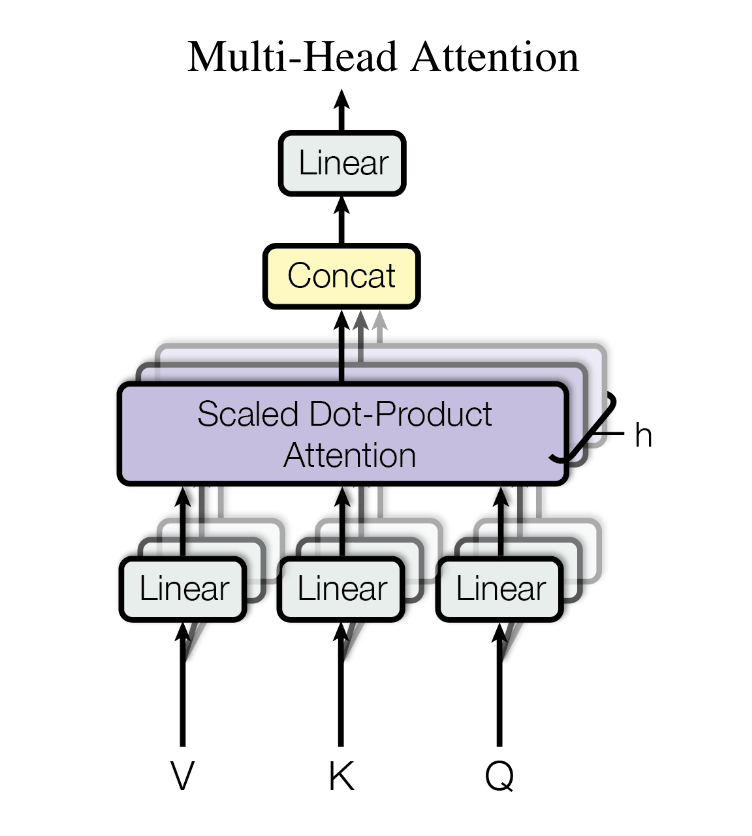
\includegraphics[width=0.6\textwidth]{figures/fig005.png}
    \caption*{Autor:\cite{vaswaniAttentionAllYou2023}}
    \label{fig:fig005}
\end{figure}

O mecanismo de atenção é particularmente chamado de ``Atenção de Produto Escalar Dimensionado'', visto na Figura \ref{fig:fig005}. A entrada consiste em \textit{queries} e chaves de dimensão $d_{k}$ e valores de dimensão $d_{v}$. São calculados os produtos escalares da consulta com todas as chaves e dividido por $\sqrt{d_{k}}$, para fins de controle dos valores em uma menor amplitude. Em seguida, aplica-se uma função \textit{softmax} para obter as probabilidades sobre os valores. Na prática, é calculada a função de atenção em um conjunto de consultas simultaneamente, agrupadas em uma matriz $Q$. As chaves e os valores também são agrupados em matrizes $K$ e $V$. Calcula-se a matriz de saídas como:

\begin{equation}
\text{Attention}(Q, K, V) = \text{softmax}\left(\frac{QK^T}{\sqrt{d_k}}\right)V
\label{eq:attention}
\end{equation}

Dentre os pontos de vantagem do mecanismo de atenção, se destacam: o total de poder computacional por camada, o total de computação que pode ser paralelizada e o poder de capturar a relação de dependência entre dados que se encontram distantes espacialmente um do outro. Como benefício adicional, o mecanismo de atenção pode gerar modelos mais interpretáveis, sob o ponto de vista de como os \textit{tokens} se correlacionam. Não apenas as cabeças de atenção individuais claramente aprendem a executar diferentes tarefas, muitas parecem exibir comportamentos relacionados à estrutura sintática e semântica das frases, no caso da aplicação em \textit{tokens} oriundos de textos.

%--------------------------------------------------------
\section{OTIMIZADOR ADAM}
\label{sec:adam}

Toda rede neural é treinada aplicando otimização em uma determinada função objetivo afim de minimizar o erro perante os dados de treinamento. Neste contexto, o presente trabalho escolhe o \gls{adam} como otimizador dada sua adaptatividade.

O método \gls{adam}, introduzido por \citeonline{kingmaAdamMethodStochastic2014}, é um método popular para o treinamento de modelos de \gls{ap}. O \gls{adam} combina os benefícios de outras duas técnicas de otimização, o \textit{AdaGrad} e o \textit{RMSProp}. O \gls{adam} é um método de otimização estocástica eficiente que requer apenas gradientes de primeira ordem com pouca exigência de memória. O método calcula taxas de aprendizado adaptativas individuais para diferentes parâmetros a partir de estimativas dos primeiros e segundos momentos dos gradientes.

Algumas das vantagens do \gls{adam} podem ser elencadas: taxas de aprendizado adaptativas, que levam a uma convergência mais rápida e eficiente se comparadas com métodos de aprendizado fixos; robustez, que suportam gradientes esparsos de forma efetiva, cruciais para diversas aplicações de \gls{ap} atuais; fácil de utilizar, pois requer menos ajustes de parâmetros a tornando amigável ao usuário e acessível a uma grande gama de tarefas.


% Capítulo 3 - Conclusão
% ---
%% USPSC-Cap3-Conclusao.tex
% ---
% Conclusão
% ---
\chapter{Conclusão}
\vspace{-\baselineskip} %Manter para garantir o espaçamento da biblioteca.
% ---
% O comando abaixo insere parágrafos aleatórios só para exemplificar
Apresentar as conclusões correspondentes aos objetivos ou hipóteses propostos para o desenvolvimento do trabalho, podendo incluir sugestões para novas pesquisas.


% ---


% -----------------------------------------------------------
% Referências bibliográficas
% ----------------------------------------------------------
\bibliography{FEI-bib/modelo-references}


% ----------------------------------------------------------
% Apêndices
% ----------------------------------------------------------
%% USPSC-Apendice.tex
% ---
% Inicia os apêndices
% ---

\begin{apendicesenv}
% Imprime uma página indicando o início dos apêndices
%\partapendices

 
\chapter{O que é Apêndice}
\vfill
\clearpage

Elemento opcional, que consiste em texto ou documento elaborado pelo autor, a fim de complementar sua argumentação, conforme a ABNT NBR 14724 \cite{nbr14724}.

Os apêndices devem ser identificados por letras maiúsculas consecutivas, seguidas de hífen e pelos respectivos títulos. Excepcionalmente, utilizam-se letras maiúsculas dobradas na identificação dos apêndices, quando esgotadas as 26 letras do alfabeto. A paginação deve ser contínua, dando seguimento ao texto principal. \cite{aguia2020}
% ----------------------------------------------------------
\chapter{Exemplo de tabela centralizada verticalmente e horizontalmente}
\vfill
\clearpage
\index{tabelas}A \autoref{tab-centralizada} exemplifica como proceder para obter uma tabela centralizada verticalmente e horizontalmente.
% utilize \usepackage{array} no PREAMBULO (ver em USPSC-modelo.tex) obter uma tabela centralizada verticalmente e horizontalmente
\begin{table}[h]
\ABNTEXfontereduzida
\caption[Exemplo de tabela centralizada verticalmente e horizontalmente]{Exemplo de tabela centralizada verticalmente e horizontalmente}
\label{tab-centralizada}

\begin{tabular}{ >{\centering\arraybackslash}m{6cm}  >{\centering\arraybackslash}m{6cm} }

\hline
 \centering \textbf{Coluna A} & \textbf{Coluna B}\\
\hline
  Coluna A, Linha 1 & Este é um texto bem maior para exemplificar como é centralizado verticalmente e horizontalmente na tabela. Segundo parágrafo para verificar como fica na tabela\\
  Quando o texto da coluna A, linha 2 é bem maior do que o das demais colunas  & Coluna B, linha 2\\
\hline
\end{tabular}
\fonte{ Autores}
\end{table}

\end{apendicesenv}
% ---

% ----------------------------------------------------------
% Anexos
% ----------------------------------------------------------
%% USPSC-Anexos.tex
% ---
% Inicia os anexos
% ---

% Imprime uma página indicando o início dos anexos

\begin{anexosenv}
% ---
%\partanexos
\noindent \chapter{Exemplo de anexo}
\vfill
\clearpage
% ---
Elemento opcional, que consiste em um texto ou documento não elaborado pelo autor, que serve de fundamentação, comprovação e ilustração, conforme a ABNT NBR 14724. \cite{nbr14724}.



\noindent\chapter{Acentuação (modo texto - \LaTeX)}
\vfill
\clearpage
\begin{figure}[H]
	
	\caption{\label{fig_anexob}Acentuação (modo texto - \LaTeX)}
	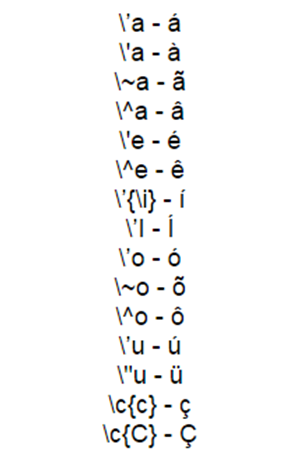
\includegraphics[scale=1.0]{imagens/USPSC-AcentuacaoLaTeX.png} \\
	%Fonte: \citeonline{comandos}
	Fonte: \citefonte{comandos}

\end{figure}

\end{anexosenv}


\end{document}
